\documentclass[11pt,a4paper,smallheadings,cleardoubleplain,DIV10]
{scrbook}
\usepackage{pyblio,natbib}
%\includeonly{td-rg3}
% add font styles  like: ,galliard,gillsans, if you like
\hyphenation{data-base}
%\rcsInfo $Id$
\externaldocument[DG.]{DG}
\externaldocument[RM.]{RM}
\begin{document}
\frontmatter
\title{Pybliographer User's  Guide}
\author{Fr�d�ric Gobry and Peter Schulte-Stracke}
\maketitle{}
\tableofcontents

\mainmatter
\pagestyle{headings}
% \begin{abstract}This manual gives an introduction and reference for
%   the use of Pybliographer version 2.
% \end{abstract}

%%% ad interim 

\reversemarginpar

% Part 1 -- Introduction
\part{Introduction}

\chapter{A Primer for Pybliographer}
\label{cha:rgintro}


This chapter provides an introduction to \Pyb\ for new users.
If you are already familiar with \Pyb, you can skip this chapter.


% Bibliographic database managers are a specialized type of a database
% manager designed for the handling of bibliographic references. They
% are also known as personal information systems, bibliographic
% reference managers, or personal bibliographic software. These systems
% help with three essential research tasks:

%  *  Building a database of references to journal articles, books, and
%     other research publications, using both manual and electronic
%     input methods 
%  *  Searching the created database by author, subject, journal name,
%     and other criteria 
%  *  Generating a list of selected references from
%     the database in a specified format for various purposes

% Options for managing references and other textual information
% -------------------------------------------------------------
%  *   Card based paper index 
%  *   Generic flat file database, e.g., PC File 
%  *   Generic relational database, e.g, MS Access, Paradox, DBase. Some
%      of these will also allow you to include graphics as well as text. 
%  *   Textual database manager. The more generic programs allow one to
%      organize and index text of varying sizes. 
%      AskSam is a leading example of a generic textual database
%      manager. Bibliographic database managers are a
%      customized form of this type of software. See Features of
%      Bibliographic Managers below.  

% Uses of Bibliographic Database Managers
% --------------------------------------------------

%  *   Create course reserve lists and reading lists for students 
%  *   Maintain faculty publication lists 
%  *   Catalog special collections 
%  *   Keep track of reprint collections 
%  *   Maintain bibliographies of references in research areas of
%      personal interest  
%  *   Prepare instantaneous formatted in-text citations and
%      bibliographies during manuscript preparation  
%  *   Create and maintain a reference database shared among a group of
%      resources across a network  
%  *   Publish a web-based bibliography 


\section{How Pybliographer can Help You}
\label{sec:whyuse}




Pybliographer provides Reference manager services to create, load,
modify, list, read, transport, and copy description of resources like
books, articles, and electronic documents, including derivative and
private information.



% [[Many restrictions inherent in the  BibTeX database format used by
% earlier versions of this program are removed or relaxed in this
% version. 

% This version continues to support \BibTeX\ databases to assist you in
% converting to the new database structure. [XXX Subsequent releases,
% however, might not support these features, so we strongly recommend
% conversion to the exclusive use of the new database structure.

% Support for using \BibTeX\ as an import and export format only,
% however, is planned for the foreseeable future.] 
% ]]


To introduce you to the use of \Pyb, we consider three scenarios or
\textit{workflows} first.  Each of these scenarios represents a basic
usage context for the application. In the following they are presented
in sequence of increasing complexity, so that each one is, in fact,
included in the next.



\subsection{Scenario: Search and Browse}
\label{sec:search-browse}

Searching information is certainly the most fundamental (also the most
frequent) task for a reference manager database.  You can look up
records in a variety of ways, starting from whatever information you
have.  There are two ways to start a search, (i) by entering
\textit{search terms}, be it words or \textit{regular expressions}, or
(ii) alternatively by \textit{selecting index terms} from a list.
This list can be a comprehensive index of, e.g., persons taken from
the whole database, or the result of an operation; so you can
effectively follow the associations from article to person to other
article and so on.


\label{sec:workflow1}
In general the searching can be subdivided into the following stages
and tasks:

\begin{table}[htbp]\sffamily\small
  \begin{tabular}[t]{|l|p{10cm}|}
\hline \textbf{Stage}& \textbf{Description}\\ \hline
\textbf{1}& Choose a database, \textit{if necessary}\\
\textbf{2}& Do a \textit{Known-Item-Search}, e.g., with an author\slash
title pair, \textit{or}\\
\textbf{3}& \textit{Browse an Index}, if you are looking for things you
   don't know beforehand (or might have forgotten), e.g., in a Journals
   Index, \textit{or}\\
\textbf{4}& Follow a cross-reference, e.g., by looking at the works of an
   author, or papers which cite another, \textit{or}\\
\textbf{5}& Based on the results, variate or make more precise the search
   question, or even\\
\textbf{6}& Formulate an \textit{expert query}, this requires some
   acquaintance with the data base.\\
\textbf{7}&  \textit{Look over the results.} Examine individual
records. \\
\textbf{8}&  Mark items to set them aside for further examination or
   processing.\\
\textbf{9}& Add a note  to an item.\\
\textbf{10}& Output all or any of the items, in various formats, to another
   file, to the clipboard for inclusion in another document
   (using \textit{Drag-and-drop}), to the printer. \\
\hline
  \end{tabular}
  \label{tab:workflow1}
\end{table}

\newpage

\subsection{Scenario: Write a Paper}
\label{sec:workflow2}

Within the following scenario, you will find yourself searching and
browsing (as above in \ref{sec:search-browse}) many times; now these
\textit{Use Cases} are imbedded in more complex processes. So, e.g.,
stages 6 and 7 below consist not only of searching and browsing
activities, but integrate them with the writing process: an item is
not only found, but it's citation is included in the document in
preparation, it is placed on or taken from a work list, a reference is
linked back to the cited item etc.

\begin{table}[htbp]\sffamily\small
  \begin{tabular}[t]{|l|p{10cm}|}
\hline \textbf{Stage}& \textbf{Description}\\ \hline
&\textbf{Collect Information}\\
\textbf{1}& Maintain a reading list.\\
\textbf{2}& Acquire information from databases.\\
\textbf{3}& Acquire information from other sources.\\
\textbf{4}& Add notes and quotes.\\
& \textbf{Write}\\
\textbf{5}& Maintain a work plan.\\
\textbf{6}& Find items, notes, quotes, etc.\\
\textbf{7}& Insert and mark-up references and quotes.\\
\textbf{8}& Audit work done. (Check cited works, etc.)\\
\textbf{9}& Process references for output formatting.\\
\hline
  \end{tabular}
  \label{tab:workflow1}
\end{table}

\subsection{Scenario: Maintain a Bibliography}
\label{sec:workflow3}

The linking process that lies at the core of \Pyb's support of the
writing process is applied in the next, most demanding situation to
documents of various kinds that are \textit{given} and
\textit{augmented} for better analysis and access.
% Now consider another  situation, where you want to build and maintain
% a website devoted to your favourite writer, A.U.~Thor.   Of course,
% you will want to make maximum use of your computer and derive the
% web presentation from the database. \dots

% A special need is to keep track of things coming in.
% Take reviews, which must be somehow related to the subject work \dots


\begin{table}[htbp]\sffamily\small
  \begin{tabular}[t]{|l|p{10cm}|}
\hline \textbf{Stage}& \textbf{Description}\\ \hline
\textbf{1}& Organise work.\\
\textbf{2}& Add and import records.\\
\textbf{3}& Check, edit and merge records.\\
\textbf{4}& Add documents.\\
\textbf{5}& Describe (mostly) archival items and collections.\\
\textbf{6}& Maintain authority data. \\
\textbf{7}& Add and edit access points.\\
\textbf{8}& Add annotations, other texts.\\
\textbf{9}& Process output.\\
\textbf{10}& Export data for backup, integration.\\
\hline
  \end{tabular}
  \label{tab:workflow1}
\end{table}



% An example scenario follows:

% Let's consider a simple situation first.  During a talk with a friend,
% you suddenly remember a paper that you read a while ago.  Back home,
% you look it up in your Pybliographer Database:

% In the Search Window (Fig. \ref{fig:searchx1}) you enter the author name and
% a word from the title (other approaches are possible and are discussed
% in section XXX):

% \begin{figure}[htbp]
%   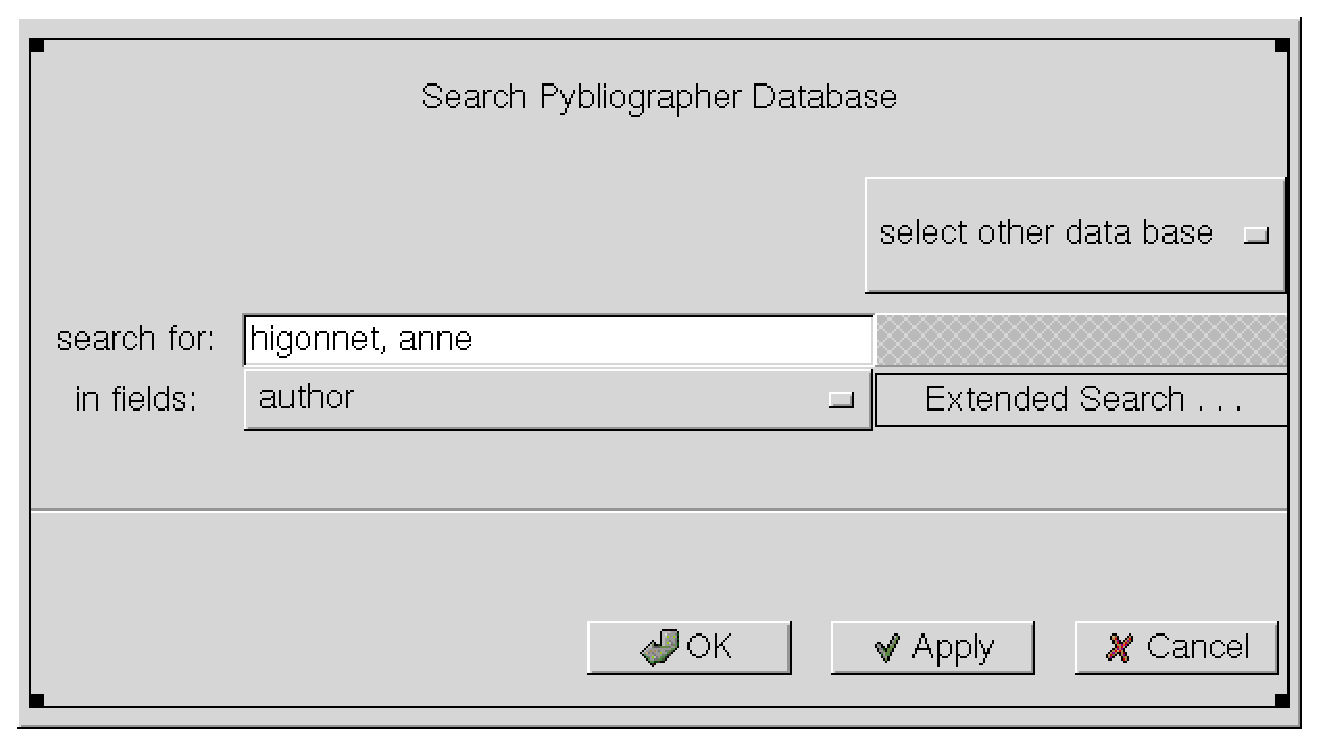
\includegraphics[width=.6\textwidth,bb=0 0 617 342]{pics/searchx1.eps}
%   \caption{Search window with example search terms entered.}
%   \label{fig:searchx1}
% \end{figure}


% The system replies by displaying the list of one item found, and also
% the first and only item in a subwindow (Fig. \ref{fig:searchx2})

% \begin{figure}[h]
  
%   \caption{Display of example search results}
%   \label{fig:searchx2}
% \end{figure}

% You decide to e-mail the citation to your friend. You can easily
% insert it into the e-mail with the standard \textit{drag-and-drop}
% mechanism that Pybliographer supports. The format of the citation is
% easily selected and changed (XXX).

% Perhaps you should try and look for some other references in this area
% when your are in the library again? Let's attach a note to the item,
% so as to be reminded of it when you visit the library the next time: 

% \begin{figure}[ht]
  
%   \caption{Adding an action note}
%   \label{fig:searchx3}
% \end{figure}


% \subsection{Writing an article}
% \label{sec:writing-an-article}

% \label{sec:workflow2}
% \begin{enumerate*}
% \item 
% \end{enumerate*}

% It's only a short note this time, so we don't need much preparation. A
% review say, the book lays on your table, a couple of notes, the editor
% is started. You didn't enter the book into your database yet, so you
% start with querying your national library (see Fig.~\ref{fig:searchx4}
% ). This has the useful side effect of telling you whether the author
% in question has already published something (no need to put your foot
% in it).

% \begin{figure}[ht]
  
%   \caption{Looking up an author in an external database}
%   \label{fig:searchx4}
% \end{figure}

% Whenever you look something up in this way in an \textit{external
%   databaese}, as opposed to the Pybliographer database, the result of
% your query will be captured in an internal list, it is then available
% for further processing, but not yet entered into the Pybliographer
% database. The reason for this is, that it may be too much work for the
% moment -- and it is work that must be done diligently -- to check-in
% and adapt each an every item that a database query might deliver. (See
% the next chapter, in particular ... for more information on this.)
% But in this case, there are but two items, which are easily added.

% If the information comes, as it is here presumably the case, from a
% Z39.50 connected and MARC serving database, there is usually little to
% do at this stage. One point, however, remains to do: the new entries
% must be correctly categorised, lest our fine arrangement goes to
% pieces. If we are content with the standard folder mechanism, it
% should suffice to travers the folder hierarchy until the right leave
% is found, then to drop the item(s).

% \begin{figure}[ht]
  
%   \caption{Dragging an item into a folder}
%   \label{fig:searchx5}
% \end{figure}
 
% To commence the article, you drag the corresponding item on the editor
% window and drop it there: the formatted bibliographical reference is
% inserted and easily edited by you for publication.

% You follow this first paragraph by your observations, occasionally
% consulting your paper notes perhaps. Oh, and this paragraph on page
% 123 you would like to quote, but first you enter it in Pybliographer's
% quotation storage. (XXX) A new editor window appears and already knows
% the item from which you want to enter the text. It first asks you for
% the page number, so you cannot forget it, and then lets you enter and
% edit the text. 

% \begin{figure}[ht]
  
%   \caption{Entering a quotation}
%   \label{fig:searchx6}
% \end{figure}

% By simply dragging the quote into the editor window you not only get
% the text, but the citation as well. You decide to use only a portion
% of the full quote, so you delete a portion of it. Then you want to add
% another voice, whatever was his name \dots\ You decide to open the
% author list and position it at the approximate name.

% \begin{figure}[ht]
  
%   \caption{Displaying the author list}
%   \label{fig:searchx7}
% \end{figure}

% You select and open the right entry (let's assume this), and
% look down the list until you find the wanted entry. From the detail
% view of this entry you could again choose a quote, but then you
% decide otherwise, and simply cite this article instead, you already
% guess, how to do it.

% \begin{figure}[ht]
  
%   \caption{Citing an item}
%   \label{fig:searchx9}
% \end{figure}

% Let's stay for a moment yet with the detil view: the article had been
% quoted, you remember, and selecting the references view lets you find
% this article as well. A sentence from here would fit in much better
% with you review, wouldn't it? 

% \begin{figure}[ht]
  
%   \caption{Excerpt -- sections and quotes}
%   \label{fig:searchxa}
% \end{figure}

% When you are finished with your work, Pybliographer does the
% bibliography for you, simply select Format/references from the
% Menu. You need to specify a stylesheet, and some other options, and
% then you can lay back and relax.

% \begin{figure}[ht]
  
%   \caption{Dialogue Formatting options}
%   \label{fig:dlformat1}
% \end{figure}



% \subsection{Maintaining a Web-Site}
% \label{sec:howwebsite}

\newpage
\section{Bibliographic Records in Pybliographer}
\label{sec:showbibrec}


\begin{dnote}
  \item Show a record display here for entertainment
  \item Explain major UI elements (1 page)
\end{dnote}

%\newpage

%%%%% this table logically pertains to next section

\begin{table}[htbp]\sffamily\small\leftskip-2cm
  \begin{tabular}[t]{|p{8cm}p{8cm}|}
\hline \textbf{Description}& \textbf{Examples} \\
\hline
\textbf{Bibliographical Description}\par
 According to ISBD, this comprises the title and statement of
 resposibility area, the edition area, the materials specific area, the
 publication statement area, the physical description area, the series
 statement area, the notes area, and the standard numbers and terms of
 availibility area.
 &
 {\obeylines
 +Der+ Zauberberg / Thomas Mann
 A l'ombre des jeunes filles en fleurs / Marcel Proust
 [kit] [motion picture] [art original] 
 31. Aufl. \quad In full score 
 Vol. 1, no. 1 (winter 1957)-
 Scale 1:3,500,000
 Amsterdam: N. Israel, 1973
 vi, 754 p. : ill. (some col.); 24 cm
 (Actualit\'es scientifiques et industriels; 1236)
 Thesis (Ph.D.) -- University of Michigan, 1971
 Includes Indexes
 }\\
\textbf{Access Points}\par
This is information that characterises the item in terms which are,
generally speaking, not taken from the item, at least not verbatim.
Using a controlled vocabulary is als known as authority control, lists
of such terms are called authority files.\par
Names of persons and corporate bodies are (for the orthodoxy) the most 
important access points, and pose characteristic problems. Other types
of data in this class are subject headings, classifications, keywords
and uniform titles.
&{\obeylines
Albertus <Magnus>
Montherlant, Henry +de+ 
Alvarez Quintero, Seraf\'in, 1871-1938
Paulus <Apostolus>: Epistolae ad Thessalonicenses
Deutscher Biologentag <6, 1964, Hersfeld>
Programming languages (Electronic computers)
30 A 58 \quad D.3 \quad 11103-57-4 (Vitamin A)
EC 4.1.3.1 (isocitrate lyase) 
}\\
\textbf{Contents related information}\par
This includes all information taken from the item at hand, be it
transcribed verbatim or not.
&
{\obeylines
Abstract
Short summary note
Quotation
Excerpt
ad-hoc keyword
}\\
\textbf{Task related data}\par
This information is used to keep track of various tasks associated
with the reading and using of resources. 
&{\obeylines
Project/reading list
Desiderata
Orders (bookseller, inter-library loan)
Items by location (library, shelf)
}\\
\textbf{Holdings information}\par
Information that is neccessary to gain access to an item
&
{\obeylines
URL \quad file name 
Call number \quad Shelf number 
Institution (library) code
Shelving place, binder (for copies)
}\\
\hline
    \end{tabular}
  \caption{Information stored in a reference manager}
  \label{tab:knorrtyp}
\end{table}
\newpage
\section{Describing Resources}
\label{sec:introdesc}
\nopagebreak
\begin{dnote}
  \item Give an overview of the requirements for various user
    situations (cf. Eversberg, ...)
  \item Introduce to the Chapter 3 treatment of planning decisions
    w.r.t. level of description, use of classifications, \textit{rigeur}
  \item Background for daily work, giving overall direction. 
\end{dnote}
Before we can search for them, the resources of interest must be
identified and described. \dots 
\begin{itemize*}
\item To identify
\item To distinguish
\item To access
\end{itemize*}





\subsection{A Model of Bibliographical Data}
\label{sec:introdata}

A model of the data that is relevant for our application (taken from
Knorr \citep{knorr98}) is shown in Table \ref{tab:knorrtyp} on page
\pageref{tab:knorrtyp}.


% \label{sec:introacc}

% Not infrequently we might want to a little reading. \Pyb\ can help us
% here in many ways:
% \begin{itemize*}
% \item By searching for a title -- looking for holdings information
% \item By providing on-line access
% \item By helping organise our work
% \end{itemize*}




% \section{General considerations}
% \label{sec:descgen}


% When describing ressources of any kind, we encounter some problems
% again and again. 

% The first has to do with the question which information to use; more
% specifically where to look for the information.

% To reduce the variation and confusion when describing ressources, there
% are certain established principles, among others:

% \begin{itemize}
  
% \item Use the original text, if possible. This principle avoids e.g.,
%   the confusion arising from giving a place of publication that is
%   \textit{K�ln, C�ln, Keulen, Cologne}, depending upon time and place
%   of cataloguing. 
% \item Use special normalised forms to account for the needs of users
%   that might not know the original form, but do not replace the
%   original form (for important pieces of information), but give both
%   of them.
% \item Prefer the information as it is found on the title page (and
%   some comparable places).  At least indicate information that does
%   not come from the standard places by putting it into brackets [].
% \item Distinguish the various classes of information, in particular do
%   not confound formal and material description, nor bibliogrpahic
%   description and annotations etc. although the software supports it
%   both. It much simplifies life to keep these purposes apart.
% \end{itemize}


\section{Exploiting [Working with] Resources}
\label{sec:introexpl}

We do not acquire, store, and browse bibliographical records for their
own sake, but in order to put them to use.  For at least as long as we
are sitting at our thesis it is our daily task to use them and we
want to make the most of them, and of the fatures that  \Pyb\ offers.

The most basic use is, of course, citing a source. Often that includes
taking a quote from it. Then we might want to obtain a list of cited
works (references), but also need support for our work in form of list
of references eyemarked, or already used, or yet to be considered. It
is furthermore helpful to be able to flexibly handle quotations.\dots

Often our memory is not quite up to the task and we want assistance in 
using sources, tha \Pyb\ happily provides. It allows us to store
quotes, to add notes, even longer excerpts and reviews, if we want. We
can not only cite them comfortably, but also search them without
regard to their being stored within or out of the database proper. 

Finally, if our work continues for a while, we may find the many ways
useful, that \Pyb\ provides to \textit{organise} the database. So we
can ask for \textit{subjects} by means of attaching subject headings
or classification codes, we can trace editions and reviews of or
references to a work, and we can keep track of our own work.


\section{Special Materials}
\label{sec:introsmd}


Many reference managers are geared towards the formatting of
references most frequent in scientific\slash technical papers, almost
as much as library type applications are towards the cataloguing of
monographs.

In contrast \Pyb\ tries to be adaptable and extensible enough to
support the specialist, while not losing its usability for the average
user (which the specialist remains to be, after all, outside of his
area of specialisation).

What does that mean? \Pyb\ provides an extensible, open, and adaptable
database schema, and appliction programming interface (API).  More
about extending and adapting \Pyb\ can be found in chapter
\ref{cha:pscript}.  An interface alone, however is not sufficient. 
Of equal or possibly even greater importance is a sound database
structure, something missing from most popular alternatives. More
about the database structure you can find in section \ref{sec:rgccont}.

In the following a number of specific requirements are detailed,
together with an indication of what \Pyb\ does offer you in that
respect.

\begin{description}
\item[Archival and administrative records] need a different treatment
  because they are unique, depending on context (provenance) for
  description, access, and interpretation.  Thus they require a
  multi-level description, as item but also on the collection level.
  In addition, they often form series, that warrant structured
  annotations for analysis, \dots
\item[Continuing resources, collections] include serials, journals,
  web-sites, e-journals, and the like (user-maintained, so-called
  artificial collections are similar enough to warrant mention here).
  The degree of \textit{description} that is usually needed varies
  considerably, what is important, however, is the support \Pyb\
  provides for not-so frequent situations.
\item[Multi-level description] is generally available and helps with
  handling of articles in journals (journal data are stored and
  maintained separately) monographs in series, documents on web-sites, 
 and so on.
\item[Analytical annotations] add to the annotation facilities with
  the option of form-based or tabular data entry.  Typical situations
  are preparation of meta-analyses or historical case
  analyses. (Example \dots) (This is really a requirements statement
  XXX)
\item[Music] is supported by (i) multilevel description for, e.g.,
  sound recordings, where more than one piece is on one carrier, and
  (ii) by handling \textit{works}, allowing searching and displaying
  of multiple recordings but also manuscript or printed scores,
  etc. 
\item[Audio and Video Recordings] and many other materials can be
  correctly described  
\end{description}

\begin{dnote}
\item This section should alert the user to the fact that the needs of
  particular kinds of materials are looked after, -- and that there
  are such special needs.
\item I would rather like a table: Material -- Problem -- Solution
\item Cf. AACR2R for a list of special materials (and \textsf{MARC 007})
\end{dnote}

\section{Special Needs}
\label{sec:introspecial}

\begin{dnote}
  \item More processing related questions?
\end{dnote}



%%% Local Variables: 
%%% mode: latex
%%% TeX-master: "UG"
%%% End: 


\chapter{Pybliographer Concepts}
\label{cha:rgconc}

This chapter summarises some basic concepts that you need to
understand before you can use \Pyb.
It briefly describes:
\begin{itemize*}
\item What bibliographic items are and how they are described
\item What basic data types are used 
\item How the data is stored and processed
\item How \Pyb\ can help you storing and editing bibliographic
  resources and using them in you work
\end{itemize*}


\section{The Content of the Database}
\label{sec:rgccont}

The \Pyb\ database contains records of many types.  The following main
classes can be distinguished: 
\begin{itemize*}
\item Records that contain classifying information \textit{in the
    widest sense}, and which are loosely called \textsf{\itshape
    Topics}, as they are subclasses of \textsf{Topic}.
\item Records that contain the bibliographic description proper
\item Records that contain additional data, loosely called
  \textit{annotations}.
\item Internal records, containing \textit{configuration objects}.
\end{itemize*}



\subsection{Informations that Structure the Database}
\label{sec:rgconctopic}

The information that we speak about in this section represent a
concepts of bewildering variety -- however they all serve the common
purpose of organising the \textit{payload} of the database and share a
common technical base.

\begin{description}
\item[Classifiers: Languages, Genres, Forms, etc.] Without doubt, this
  is the least difficult kind of data used in connection with
  bibliography.  We have no taxonomic (tree-like) structure, but only a
  linear list of possible values, and mostly but little in way of name
  variants (\textit{see} references), only the need for translations of
  the list entries are a small complication that implies a little by
  way of programming.
  
  In most cases, such values are not \textit{indexed} in the sense
  that a list of items such as those that fulfil ``Language = XYZ'' is
  maintained by the system.  A query for all such items is then 
  necessarily done by scanning the whole database.  See
  \ref{sec:rginstcodes} for more informations.
\item[Keywords, Descriptors] Look similar but are very different
  because they do not come from a (mostly) pre-defined set.  That
  makes a difference not only for the programmer, but also for the
  user -- the longer list is not as easy to overview, see
  \ref{DG.sec:orgkeys} for a discussion of keywords.
  
  Open-ended lists occur also in connection with externally defined
  descriptors, such as the enzyme (EC) numbers. These are considered
  classifications (degenerate, if they do not form a tree, v. infra).
\item[Subject headings] on the other hand have a \textit{taxonomic}
  structure, they are linked to permit navigation to and from broader
  and narrower terms as well as related or opposite terms.  This comes
  at a price (no surprise) and most users will content themselves with
  what external databases provide.  Note, however, that \Pyb\ comes
  with a relatively sophisticated model of subject headings, which you
  could use to your profit by mapping incoming externally defined
  values to the preferred set, if you have one available for your area
  of work. 
\item[Classifications] The other generally used means of adding
  subject information to bibliographical records is by classifying the
  items described.  A classification, as e.g., the Mathematical
  Subject Classification \citep{MCS2000} comes as a tree where usually
  the leaves are eligible classes.  One typical property of
  classification is the use of codes (notations) to represent the
  classes, so is, e.g., \textsf{14G35} the code for ``Modular and
  Shimura varieties'' in the MCS with note ``[See also \textsf{11F41,11F46,
  11G18}]'' added. 
\item[Persons, Corporate Bodies] Persons or names of persons, and also
  corporate bodies, are well-recognised entities in library systems
  since long; this has not been the case for reference manager
  applications.  It is, however, obvious that they profit as well. 
\item[Works, Expressions] It has been usual, to varying degrees, to
  collect manifestations or expressions together which belong to one
  \textit{work}, so as to simplify the search and facilitate the
  selection.  It has proved even more necessary with on-line
  catalogues which are less easy to peruse.  A work is an optional
  element in that the average item has no need for it (it could be
  considered itself work and manifestation in one, without any
  consequences following from it) and under the control of the user,
  who groups the items, if the need arises.  This replaces
  functionally the entry of a uniform title.  
\end{description}\noindent

Missing in the above are user interface elements, like folders or
lists, that equally structure the database  and group items, but  that
are not equipped with the machinery, nor have the stability (and cost)
of the above mentioned tools.

Equally missing is the venerable concept of an entry type, like
\textit{article, proceeding} or even \textit{e-mail}.  It is replaced
by a far superior scheme, that separates concerns, allows for data
entry that is adapted to your needs, and does not arbitrarily restrict
you. 

\subsection{The Bibliographical Description}
\label{sec:rgconcbiblio}

Functionally the bibliographical records could be divided into a
the description proper and annotations, logically into a core and
extensions, technically into structured and unstructured, i.e.,
textual parts.

\begin{description}
\item[Core] A bibliographical record contains minimally some
  administrative data, and a title\footnote {A missing title is
    \textit{missing}, i.e., irregular, not \textit{not applicable}.}
  more precisely a `Title and statement of responsibility area'
  followed optionally by an `Edition area' (ISBD).
  
\item[Extended description] The old description was tilted towards
  books, this is nowadays but one of the possibilities. The format
  allows any number of extended descriptions, to accommodate all
  needs. 
\item[Associations] Authors, subject and similar informations are
  considered entities, thus they are not stored in the bibliographical
  record, but only a reference is.

\item[Annotations] are textual notes (but perhaps also structured
  \textit{case annotations}) including quotes from the item. -- This
  is a mixed-up class, that could need some further elucidation.


\item[Holdings] information refers to the actual location (incl. net
  and file system addresses) of an item; it can also include a
  reproduction specification.
\end{description}



\section{Interfaces}
\label{sec:rgcintf}

For (i) accessing and (ii) for extending. 

\section{Handling Associations}
\label{sec:rgcassoc}



% \section{The Peculiarities of Bibliographical Data}
% \label{sec:rgcdata}


% \begin{dnote}  
% \item Three types of data: Tabular, Textual, Complex, plus network of
% associations. Examples
% \end{dnote}


% \subsection{Tabular Data}
% \label{sec:rgconctab}

% Most data is stored and processed as the familiar tabular type, as a
% row of data fields, each with an associated \textit{domain} of
% permissible values. The program processes these data either as
% tuples\slash lists of values or as dictionaries with named fields.

% \begin{table}[htbp]\sffamily
%   \begin{tabular}[t]{|l|p{10cm}|}
% \hline \textbf{Type}& \textbf{Description}\\ \hline
% \textbf{Address}& Any address of publisher, author, user.\\
% \textbf{User}& User decription\\
% \textbf{HoldingT}& description of institution, filing  place
%                    etc. holding copy\\ 
% \textbf{Imprint ?}& Publication statement\\
% \textbf{Collation ?}& Extent information (for printed materials
%                      only?)\\ 
 
% \hline
%   \end{tabular}
%   \caption{Data in tabular form}
%   \label{tab:tabulardata}
% \end{table}



% \subsection{Complex Data}
% \label{sec:rgcoccompl}

% A minority of data elements is better handled through a higher level
% interface.  This \textit{complex data} comprises, hawever, the most
% prominent and important data elements of bibliographic records (no
% surprise, I suppose). 

% \begin{table}[htbp]\sffamily
%   \begin{tabular}[t]{|l|p{10cm}|}
% \hline \textbf{Type}& \textbf{Description}\\ \hline
% \textbf{Names}& Personal, corporate, and names of concepts\\
% \textbf{TitleEd}& Title and edition statement\\
% \textbf{NoteT}& Notes and annotation data like quotes\\
% \hline
%   \end{tabular}
%   \caption{Data in complex form}
%   \label{tab:complexdata}
% \end{table}





% \chapter{Working with Pybliographer}
% \label{cha:rg2}

% \newcommand{\Pyb}{Pybliographer{}}

% When you work with \Pyb, you will do so most often through one of the
% following windows:

% \begin{itemize}
% \item The Search Window
% \item The Folder Window
% \item The List Window
% \item The Detail Window
% \end{itemize}

% Often you will start with the Search Window. Enter a search term and
% start a search.  (See \ref{fig:searchx1}) The same window allows you to
% query another (possibly remote) database, and to formulate more
% complicated queries.

% Alternatively, you can open a predefined collection of records, a
% \textit{folder} or \textit{list}.  The \textit{Folder Window} allows
% you to select from all the folders and lists available. It can also be
% shown permanently as a left sidebar. Click on the small triangle to
% the left of each entry to open or close a folder in this display. Click
% on the name to display its contents in the list window.

% A list is simply a folder that is found under the label Lists at the
% beginnign of the folder display; together with the entries Marked,
% \dots

% Whatever your way, you will sooner or later see a \textit{List
%   Window}. It shows your current \textit{selection}. Usually records
% are ordered by name of first author and are displayed in a condensed
% format. Those are options that are easily set and changed; it is
% possible to tie thses settings to a particular list; think os a
% shopping list for you rnext visit to the library, that you might like
% always sorted by location.
  
% To inspect an item it is often sufficient to point with the mouse to
% it, and have a tooltip like preview window appear. It allows at the
% same time to concisely inspect  the entry and also to preview it in a
% typical format (both can be configured, of course).  Alternatively,
% you may open the deatil view (inspector) for an item. It presents you
% with a lot of information in a notebook widget. 







%%% Local Variables: 
%%% mode: latex
%%% TeX-master: "UG"
%%% End: 


\chapter{Preparing to Use Pybliographer}
\label{cha:rgprep}

This chapter discusses how to install and configure \Pyb.


It  describes how to do the following:

\begin{enumerate*}
\item Install \Pyb.
\item Set up the required database structure
  \begin{itemize}
  \item Determine which databases to use
  \item Define the directory structure or access path
  \item Define additional data that you might need
  \end{itemize}
\item Set up \Pyb\ for easier operation
\item Load needed data
\item Write local processing routines
\end{enumerate*}

Ir also discusses how much detail you will need to record, and which
standards you should consider.




\section{Installing Pybliographer}
\label{sec:rginstall}

\textbf{Note:} Before using the information in this section, you
should check the latest \texttt{Readme} file from the distribution for
any changes and additions.

As a rule, \Pyb\ installs like any other Linux program under control
of your package manager. Only in exceptional cases you will have to
consider manual installation. 

On a Debian system you use the package name \texttt{pybliographer}.So
you only need to enter
\begin{verbatim}
sudo apt-get install pybliographer
\end{verbatim}

Note that the libdb3 package will be installed, too. If you want to use
\Pyb\ together with a relational database, you must install it in
addtion to \Pyb, for more information on  using a relational
database see below. 

The following table gives the dependencies of \Pyb. [Is this a good
idea, after all?] \dots

Intructions for manually installing \Pyb.\dots


\subsection{Using a Relational Database with Pybliographer}
\label{sec:rginstdb}

When yo use \Pyb\ with a RDMS, you are in fact using a server process
in conjunction with \Pyb, which is independantly installed, configured
and started. As a rule, this server runs under a separate user
identity. Please, consult the RDMS documentation for more detailed
instructions. 

\textbf{Note:} You may want to check the considerations below in this
chapter before continuing with initialising the database.


\begin{enumerate*}
\item assure that the RDMS server is up and running, and that you have
  any necessary authorisations and informations for its use.
\item Determine the connection to the RBDS 
\item Determine the user id 
\item Start \Pyb. Open the \textsf{Application\slash Preferences} dialogue.
\item \textit{or ?} Open the \textsf{Application\slash Database} window and
  then the \textsf{Database/New} dialogue.
\item Enter the connection data, and tick the \textsf{Default
    Database} Check box.
\item \Pyb\ checks for an  existing infrastructure in the database, as
  it finds none, it alerts you that the database must be initialised.
\item Click the \textsf{OK} button on the message box.
\item The database is initialised.
\end{enumerate*}

\textbf{Note:} You may want to check the considerations in this
chapter before initialising  the database. 

 
\section{Before Using Pybliographer}
\label{sec:rginstprep}

\begin{dnote}
\item Give a task oriented overview here --
\item Refer to chapers one and two for introduction, 
\item refer to Part II for details
\end{dnote}



\section{Customisation: Codes, Lists, and Schemes}
\label{sec:rginstcodes}

\Pyb\ makes use of various lists and data bases of so called
\textit{authority data}.  See section \ref{sec:introdesc} and chapter
\ref{cha:bibl} for a discusion of authority data and the need for it.

In this section we do not address the great authority files for
persons, corporate names and the like, but the smaller  and lesser
ones that deal with codes for languages, genres, realtors et., as
follows.





\section{Customisation: Workforms, Data Entry}
\label{sec:rginstinput}

With \Pyb\ comes a standard list of \textit{work forms} that guide you
through the data entry for new records, and that are also used to
display records according to their needs. 



\section{Customisation: Import Filters}
\label{sec:rginstimport}

\Pyb\ comes with a standard set of import filters.  See
\ref{cha:uimport} for a list and discussion.   This list will suffice
in most cases for the purpose of occasional import and even when
migrating from another system. 

When the exporting system has more than one export option available,
that can be  imported by \Pyb, the results may not be equal; so you
may want to try some tests before settling for one method.

The filters provided are written so as to allow easy customisation,
extending or modifying exiting behaviour,  by subclassing them. You
may profit from this facility in the following situations:
\begin{itemize*}
\item You want to use a new format, that is a variation of an existing
  format (have a look at the examples in chapter \ref{cha:uimport}).
\item You want to use an extension of an existing format; you may want
  to make use of the additional information.
\item You want to make use of an existing format, but change the
  processing.
\item You want to make use of an existing format, and extend the
  treatment of the import data.  One such situation is given when the
  standard filter refrains from using some information because it is
  difficult to map it to the database.  You may be in able to improve
  on this situation, e.g., because you know the context.
\end{itemize*}



\section{Customisation: Output Formats}
\label{sec:rginstformat}


\section{Customisation: External Processors}
\label{sec:rginstexternal}



%%% Local Variables: 
%%% mode: latex
%%% TeX-master: "UG"
%%% End: 


\chapter{Entering Data}
\label{cha:rgnew}

This chapter discusses how you enter new data into the \Pyb\ database.
It describes:
\begin{itemize}
\item Sources and classes of bibliographic data
\item An example of creating a new record
\item Editing (modifying) data 
\end{itemize}





%%% Local Variables: 
%%% mode: latex
%%% TeX-master: "td-td2"
%%% End: 


\chapter{Searching and Selecting}
\label{cha:rgsea}

This chapter describes the steps to search and select items for
display and further processing. It shows:
\begin{itemize}
\item Possible criteria for searching and selecting
\item Ways to display the results 
\item Ways to set the results apart for further processing or later
  review 
\end{itemize}







%%% Local Variables: 
%%% mode: latex
%%% TeX-master: "td-td2"
%%% End: 


\chapter{Obtaining Output}
\label{cha:rgout}

This chapter discusses output. After an introduction it explains:
\begin{itemize}
\item Display output formatting (incl. sorting options)
\item Using drag-and-drop 
\item Fundamentals of bibliographic formatting
\item XSLT processor use
\item Output formatting choices 
\item Exporting data
\end{itemize}








%%% Local Variables: 
%%% mode: latex
%%% TeX-master: "td-td2"
%%% End: 


\chapter{Pybliographer External Interfaces }
\label{cha:extrn}

This chapter discusses various interfaces of \Pyb, including:
\begin{itemize}
\item Connections to external databases
\item Connections to other \Pyb\ databases
\item Connections to word processors and editors
\item Import and export interfaces
\item Internal application programming interface (API)
\end{itemize}

%%% Local Variables: 
%%% mode: latex
%%% TeX-master: "td-td2"
%%% End: 


% Part 2 -- Bibliographic description guide
\part{A Guide to Bibliographical Descriptions}
% \setchapterpreamble[ur]{\dictum[Thomas Hyde, \textit{Preface to
%     the Catalogue for the Bodleian Library}, [Oxford] 1674 (cited from
%   E. Svenonius, 2000, p. 9f, who in turn cites from Julia Pettee,
%   Libr. Quart. 6, 1936, 270-290, repr. in: Foundations of Cataloging,
%   1985.)]{%
%     ``What can be more easy (those lacking understanding say) having
%     looked at the title-pages than to write down the titles?''  But
%     these inexperienced people, who think making an index of their own
%     few books a pleasant task of a week or two, have no conception of
%     the difficulties that rise or realise how carefully each book must
%     be examined when the library numbers myriads of books.  In the
%     colossal labour, which exhausts both body and soul, of making into
%     an alphabetical catalogue a multitude of books gathered from every
%     corner of the earth there are many intricate and difficult
%     problems that torture the mind. }}

\chapter{Bibliographical Descriptions}
\label{cha:bibl}
\renewcommand{\dictumwidth}{.7\textwidth}
{\dictum[Thomas Hyde, Preface to the Catalogue for the Bodleian
Library, 1674]{%
  ``What can be more easy (those lacking understanding say) having
  looked at the title-pages than to write down the titles?''  But
  these inexperienced people, who think making an index of their own
  few books a pleasant task of a week or two, have no conception of
  the difficulties that rise or realise how carefully each book must
  be examined when the library numbers myriads of books.  In the
  colossal labour, which exhausts both body and soul, of making into
  an alphabetical catalogue a multitude of books gathered from every
  corner of the earth there are many intricate and difficult problems
  that torture the mind. }}
\noindent
\begin{dnote}
\item   Redundant? Cf. sections \ref{cha:rgconc},
  \ref{sec:rginstprep}, and  \ref{sec:introdesc}
\item This chapter introduces bibliographical descriptions. It discusses:
\item Purposes of bibliographical data
  \begin{itemize*}
  \item Descriptive data 
  \item Organisational data -- access points
  \item Task related data 
  \item Access providing data -- holdings  
  \item Content related data -- quotes, excerpts and electronic copies
  \end{itemize*}
\item Authenticity and authority
\item Material specific data
\item Topical data: persons, works, subjects, classifications
\item Lists of languages, genres, and similar
\end{dnote}
\noindent


Not unlike other fields of human endeavour, bibliography or
cataloguing, as it is called here for short, had needs and purposes at
its origin.  Maintaining \textit{inventories} of books that one owns,
or (more importantly) has the custody of, is certainly the earliest.
To this came certainly soon the wish to maintain \textit{directories}
of items that one might obtain, such as it happens with the
bibliographical references found in a book: they are abstract pointers
to the items detailed wheras the library catalogue contains concrete
pointers in the form of call numbers.


It is an important trait of bibliographical information to be this
kind of \textit{proxy}: Instead of looking over dusty tomes or
excavating in the basement of our memory, we push a button and query a
database.  The same applies to the references that ornate scholarly
publications, they serve not only to represent our erudition, but
also, ideally, they convey the information needed to find (although
not necessary to make good use of) the sources of our wisdom.  In this
latter case, it is necessarily so that the information must be
intelligible and usable for an `average' reader, so that it no longer
suffices to refer the reader to the `third page of the torn, slightly
greyish xerox that is near the end in the second binder on the top
shelf, left cabinet', which is how it works perfectly (and valid)
within many author's \textit{episodic memory'}.  In the following, the
question of purposes and possibilities of bibliographical data is
discussed together with some principles that are hopefully able to
guide you in deciding upon one's own special system.



\section{Cataloguing and Annotating}
\label{sec:catalog}

 
The gathering of descriptive information about bibliographical
resources is known as \textit{cataloguing}, and we use this term here
although it does not always transport the right connotations, and
distinguish it at the same time from \textit{annotating} resources.

The whole second part of this document deals not so much with
\textit{how} to do it, but with \textit{what} to do, namely
\textit{what} information to collect, where to find it, and in which
form to record it.  This reflects the importance of content in
contrast to the \textit{encoding} of this information (form), an
importance that is not always taken into account when discussing these
problems.


\subsection{Formal Cataloguing}
\label{sec:formalcat}




\subsection{Subject Cataloguing}
\label{sec:subjectcat}



\subsection{Annotating}
\label{sec:annotating}



\subsection{Integrating}
\label{sec:integrating}


\section{Some Principles and Guidelines}
\label{sec:catprinc}

It is helpful to state some principles that might direct both
programmer and user of bibliographical software (but more generally
the cataloguer, regardless of any specific programmatic support).
Part of these rules can be considered as \textit{continuity}-rules,
meaning that the result (the catalogue entry) should not vary much, if
the input (the item, the effort, the knowledge) vary but a little.


\subsection{Universality [Generality]}
\label{sec:catunivers}

\textit{The cataloguing applications (rules, tools, etc.) should be
  usable for all sorts of resources.} -- This is an important principle
that is of rather recent origin.  Historically the rules were devised
for one specific occasion and institution (only institutions had
rules).  For library catalogues, cooperative cataloguing,
inter-library loan and similar developments lead to a convergence of
rules, culminating in the \textsf{ISBD} -- but effective only only for
classical library materials (books and serials).  (The fact that the
German rules for non-book materials are somewhat at odds with the
reminder, not only weirdly reflects the sociology of the German
librarian's profession, but also the fact that they are physically
different, shelved apart etc.)

The personal computer changes this all. 
\begin{itemize*}
\item First, the focus has shifted to the desktop -- it is the
  personal bibliographical application that serves to
  \textit{integrate} the various resources and informations that its
  user needs,and this is not the program of any institution,
\item Second, the computer program requires explicit rules -- less can
  be left to (subconscious) intellectual adjustments; in addition, the
  interaction with the application stresses what is entered into the
  computer, and how -- little use is made of e.g., of the
  \textit{episodic memory} that plays so prominent a role in everyday
  life, and
\item Third, the Internet exposes the user to a great deal of
  variation -- and it's the application that must cope with it.
\end{itemize*}


Alltogether, these influences neccissitate an adaptable and multi-faceted
description format, as provided by \Pyb. (This is is true for
libraries, too.  However the span of materials is even greater in a
personal application, I suppose.) 


\subsection{Reliability}
\label{sec:catreliable}

This is another principle that only recently became evident,\footnote
{According to Eversberg.} though it underlies unstated the earlier
work as well. It has like the following one, efficiency, both a
cataloguing and a data retrieval aspect. For cataloguing (describing)
it means, that different persons should produce catalogue entries that
differ not at all, or only a little.  For bibliographical (published)
resources  this is much easier to define and control, because the
items exist in many copies; correspondingly the detail, precision, and
ambit of rules for cataloguing published, in particular printed
material by far surpass what can be said of rules for unpublished,
nmore or less unique materials. Even more this is the case for
citation guides, which ignore unpublished sources.

For published resources, there is one guiding principle, namely to
stay with what is found on the item and to transcribe it more or less
verbatim from the title page, or similarly distinguished places.





% Bibliography, not unlike other fields of human endeavour, had at its
% origins definite needs and purposes.  Originally it serves the purpose
% of maintaining inventories of items one has, as well as directories of
% items 


%%%%%%%%%%%%%%%%%%%%%%%%%%%%%%%%%%%%%%%%%%%%%%%%%%
%    DEAD 
%%%%%%%%%%%%%%%%%%%%%%%%%%%%%%%%%%%%%%%%%%%%%%%%%%




% \subsection{Library Software}
% \label{sec:introlibsw}


% This overview starts with a look at the purpose of catalogues -- the
% most important tradition to consider. 
% In 1876 Charles A.~\textsc{Cutter} thus explained the aim of the
% catalogue:\footnote{as quoted in \cite[p.196]{Hal98}}
% \begin{itemize}
% \item To enable a person to find a book of which either
%   \begin{itemize}
%   \item the author is known.
%   \item the title is known.
%   \item the subject is known.
%   \end{itemize}
% \item To show what the library has 
%   \begin{itemize}
%   \item by a given author.
%   \item in a given subject.
%   \item in a given kind of literature.
%   \end{itemize}
% \item To assist in a choice of a book 
%   \begin{itemize}
%   \item as to its edition (bibliographically).
%   \item as to its character (literary or topical).
%   \end{itemize}
% \end{itemize}

% More recently, B. Eversberg named the following main points:
% \begin{description}
% \item[Reliable search] -- this requires agreement on identifying
%   attributes and consistent data acquisition. 
%                                 % Verl��liches Finden erm�glichen

% %            "Known-item search" 
% %            Festgelegte Merkmale 
% %            Einheitliche Erfassung (Konsistenz) 
% %            Zettelkatalog: Nur 1 Haupteintragung 
% %            OPAC: Mehrere verl��liche Zugriffe 
% %            Schnelle Negativ-Feststellung 
% %            Entit�ten-Problem (Was und wer kommt in den Katalog?) 
% \item[Differentiation] between similar items (the more are in the
%   database, the more this is a problem) -- requires precise capture of
%   distinguishing characteristics of the item at hand, allows automatic
%   duplication checks.
          
% % Unterscheiden, was verschieden ist

% %            Knappe, aber genaue Beschreibung 
% %            Strikte Orientierung an der Vorlage 
% %            Haupttitelseite als prim�re Informationsquelle 
% %            Unterscheidung von Versionen eines Werks 
% %            Internationale Normierung: ISBD 
% %                 Reihenfolge und Interpunktion 
% %                 Weitgehend sprachunabh�ngig 
% %            Automatisierte Dublettenkontrolle 
  
% \item[Joining] related records may look at a first glance like the
%   opposite task. Looking closer it is best understood as a task of
%   organising references by means of equivalance classes. Typical
%   questions are for all works by one author, or all representations of
%   one work, or even all books in French or printed before 1703. Of
%   particular importance are hierarchical and derivative
%   relationsships, part of which is just usual, part of which is quite
%   uncommon (situations differ, b.t.w., take as an example the handling
%   of multi-volume works by AACR and RAK). To be sure that equivalent
%   records are not accidentally distinguished, it is often necessary to
%   standardise the description, e.g., frequently by using keywords,
%   author names, uniform titles, etc., that are taken from so called
%   authority files (Normdaten).
% % Zusammenf�hren, was zusammengeh�rt

% %            "Collocation search" 
% %            Werke eines Verfassers 
% %            Ausgaben eines Werkes 
% %            Teile von Gesamtwerken (Hierarchien) 
% %            (Werke zu einem Thema) 
% %                 Werke �ber eine Person 
% %                 Werke �ber ein anderes Werk 
% %            Ansetzung von Namen und Titeln 
% %            Normdateien 
  
% \item[Organising] search results is a problem that has yet to find
%   enough attention. Two major points are readable short titles, and
%   other display forms, and suitably designed, and enough indices for
%   browsing as well as for verification.
% % Gefundenes �berschaubar machen

% %            Ordnungsregeln 
% %            Kurzlisten 
% %            Index-Gestaltung 
% %            "Collocation search" 

% \item[Providing access] is the final purpose of all of this, and
%   nowadays it is invariably also an integrated use of the
%   bibliographical software. 
% % Gew�hltes zug�nglich machen

% %            Vom Nachweis zur Nutzung 
% %            Verbundkatalog mit Fernleih-Bestellfunktion 
% %            Zugang wichtiger als Besitz (access vs. ownership) 
% %            Finden des bestgeeigneten Exemplars 
% %            Nutzungsrechte 

% \end{description}

% % Tiefenerschlie�ung

% %       Zeitschriftenaufs�tze; Tagungsbeitr�ge

% % Mehr Wortmaterial

% %       Inhaltsverzeichnisse von B�chern; Metadaten von Verlagen?; z.B.
% %       Projekt MILOS
      
% % Integration anderer Metadaten

% %       Scan-Kataloge; Online-Ressourcen (Link-Sammlungen); z.B. EZB

% % Automatische Klassifizierung
% %       und andere neue Methoden der Sacherschlie�ung, z.B. Projekt Osiris

% % Invisible Web

% %       Datenbank-Inhalte; Volltextmaterial (PDF etc.); Inhalte von
% %       Digitalisierten Objekten Abgrenzung zur Suchmaschinen-Technik


% %%%%%%%%%%%%%%%%%%%%%%%%%%%%%%%%%%%%%%%%%%%%%%%%%%
% %  Was ist ein guter Katalog? 

% %  Nach aller Erfahrung k�nnte man ihn so charakterisieren: 
 
% %  Verl��lichkeit: hat man ein genaues Zitat, kann man schnell und mit
% %  Sicherheit feststellen, ob das Gesuchte vorhanden ist - oder da� es
% %  nicht vorhanden ist (in einem unzuverl�ssigen Katalog mu� man u.U.
% %  viele Versuche anstellen, um dies herauszufinden!)
 
% %  Zufallsfunde : in den vorhandenen Eintr�gen mu� man bl�ttern k�nnen
% %  (browsing), erstens weil oft das Ziel einer Suche nicht genau bekannt
% %  ist und zweitens weil Zufallsentdeckungen bekanntlich sehr wertvoll
% %  sein k�nnen. Deshalb gehen Nutzer zuerst ans Regal, wenn es eine
% %  systematische Aufstellung gibt. Auch der Katalog sollte daher das
% %  Durchstreifen von benachbarten Dingen unterst�tzen. Das geht im OPAC
% %  am besten durch 1.Register, in denen vor und zur�ck gebl�ttert werden
% %  kann, 2.sinnvoll geordnete Auflistungen von Ergebnismengen, und
% %  3.Hyperlinks, die direkt und schnell zu verwandtem Material f�hren.
 
% %  Tiefe der Erschlie�ung : Damit sind zwei Punkte ber�hrt, die
% %  au�erhalb der eigentlichen Katalogisierung liegen:
 
% %  1.geht es um die Entscheidung, was man eigentlich katalogisiert.
% %  Klassisch sind dies B�cher, geschlossene Pakete von Aufzeichnungen
% %  also. Oft ist es aber so, da� in einem Buch mehrere oder viele
% %  kleinere Pakete stecken, die jedes f�r sich genommen eine Einheit
% %  darstellen, nach der gesucht werden k�nnte. Man denke nur an
% %  Tagungsb�nde und Festschriften, erst recht an Zeitschriften. Im
% %  Grunde ist es in den meisten F�llen so, von Belletristik einmal
% %  abgesehen, da� ein Nutzer nur ein bestimmtes Kapitel oder einzelne
% %  Abschnitte eines Buches wirklich braucht. Katalogisiert man nur die
% %  Titel, die auf den B�chern stehen, bleiben die Bestandteile verborgen
% %  und im Katalog nicht auffindbar. Aus �konomischen Gr�nden haben aber
% %  nur wenige Bibliotheken jemals eine "Tiefenerschlie�ung" betrieben,
% %  also etwa Festschrift- oder Konferenzbeitr�ge einzeln erfa�t. Ein
% %  Spezialfall sind "mehrb�ndige Werke" mit St�cktiteln: katalogisiert
% %  man sie nur als Ganzes oder jeden Teil f�r sich (als w�re es eine
% %  Serie) oder sowohl als auch?  
 
% %  2.braucht man ein Konzept f�r die sachliche Erschlie�ung. Begn�gt man
% %  sich mit ein paar wenigen normierten Schlagw�rtern oder Notationen,
% %  um den Inhalt eines Dokuments global zu kennzeichnen, oder versucht
% %  man, wirklich jedes Thema zu erfassen, das in einem Dokument
% %  abgehandelt wird. Es gibt z.B. Experimente, bei B�chern auch die
% %  Inhaltsverzeichnisse zu erfassen, oder mit automatisierten Methoden
% %  einem Metadatensatz weitere Sachbegriffe zuzuordnen.




% \subsection{The roots}
% \label{sec:roots}



% It should prove useful to start with a view of these ancestral
% developments:

% These are still important principles, today perhaps even more than
% most of the time. 




% %In the following some of these strands are more fully discussed.


% \subsubsection[The legacy of the card catalogue -- MARC]

% \subsection{The Way of Pybliographer}
% \label{sec:way-pybliographer}



% \paragraph{Highlights of Pybliographer Release 2}
% \label{sec:highr2}
% \begin{itemize}
% \item The Index(-view) has been reworked, it now consumes less
%   resources, starts and redraws much faster.
% \item The Import facilities have been completely rewritten with a
%   view to providing a \textit{import framework}, thus much reducing
%   the expense involved in writing additional input filters, but also
%   vastly (?) improving, at the same time, the level of support and
%   comfort for every user. 
% \end{itemize}


% \paragraph{Workflow: Searching}

% A list of items is opened for inspection, or an item is searched,
% selected items are output; notes are appended, or actions requested.


% \paragraph{Workflow: Researching and Writing an Article}

% Information is collected from various sources. Entries are created and
% modified, other data is imported from the results of external database
% queries. Quotations are entered and inserted into the resulting
% document. Citations are inserted as well. A bibliography is produced
% for the document. Referenced items are recorded. 


% \subsection{Considerations}
% \label{sec:considerations}

% \subsubsection{The view from the fringes -- exotic becomes normal}



% \subsubsection{The standards evolve}
% \label{sec:standards-evolve}
% \textit{The major development has been not the Dublin Core but the
%   development of an object model that underlies the cataloguing process.}





% \subsubsection{Other lists of requirements}
% \label{sec:otherreq}



% \subsubsection{The opportunity for a flexible bibliographic format.}

% The following excerpts from a recent googling\cite{mch96} I'd like to
% add: The opportunity for a flexible bibliographic format -- Designing
% a bibliographic format for highly varied levels of effort:

%   \begin{quote}
%     It should be possible to create a bibliographic format which
%     permits people to use exactly the level of detail they wish,
%     rather than requiring or preventing less or more.  This would
%     reduce the current undesirable proliferation in bibliographic
%     formats.
%   \end{quote}


% \paragraph{The problem:}
% People create bibliographic records with enormously varying levels of
% effort.  Further, the distribution of effort across different aspects
% of bibliographic information also varies.  Current bibliographic
% formats tend to be useful only over a relatively narrow range.  They
% establish minimums by requirements on information and its form.  They
% establish maximums by limitations in the expressiveness of the format.
% They do not gracefully handle attempts to get by with less work, or to
% add more work to further refine the record.  This is approximated by
% optional fields, but the format and meaning of a fields content is
% usually inflexible.  Thus there is an undesirable proliferation of
% formats, a new one created whenever someone wants a new tradeoff in
% ease versus precision.  The new format is generally as inflexible as those
% which preceded it, and the problem thus continues. [\dots]



% \paragraph{The opportunity:}
% Create a bibliographic format which can gracefully handle a wide range
% of cataloguing intensity.  One which could handle the complete spectrum
% from Bib/Refer to MARC.  And do it in a way which permits work to be
% spent only and exactly where one wishes.  Such a format would be a
% `lingua franca', as any other bibliographic format could be converted
% into it without losing, or requiring additional, information.[\dots]


% \newpage
% \subsection{Summary of Requirements}
% \label{sec:summrequ}

% \begin{enumerate}
% \item \textit{Identifying}
% \item \textit{Organising}
% \item \textit{Accessing}
% \end{enumerate}


% \begin{itemize}
% \item The oldest stems from the librarian's duty to keep inventories
%   of his collection in form of \textit{catalogues} -- and the
%   associated application software.
% \item Very early the scholarly (and technical) document preparation
%   has been supported with programs to augment document sources with
%   correctly formatted references (\textit{Refer} and \textit{BibTeX}
%   are two similar programs for the major document processing
%   environments).
% \item These programs concerning themselves, however, only with this
%   last step, other tools developed over time to help with organising
%   and searching the databases these programs require. Such
%   \textit{reference managers} also aided in the odious task of
%   actually creating (i.e., typing) the needed entries.
% \item With the growth of Internet usage, it became possible and more
%   or less usual to access databases of bibliographical interest
%   directly. Both the nature of the data (format, extent, correctness,
%   completeness) and of the means of access (protocols, navigation,
%   access restrictions, formatting)  vary enormously. Nevertheless, it
%   has become desirable to easily integrate the results of these
%   searches into one database -- adding a new complexity to the tasks.
% \item In addition, more and more the exchange of documents needs to be
%   integrated, too. 
% \item The World Wide Web may also serve as an imperfect but easily usable
%   and ubiquitous way of providing \textit{access} to a database.
% \item Finally, the traditional library catalogues have also added
%   support for additional administrative functions (both on the
%   acquisitions as on the lending side), many of which are quite
%   natural extensions of their primary function.
% \end{itemize}







%%% Local Variables: 
%%% mode: latex
%%% TeX-master: "UG"
%%% End: 


\chapter{Persons, Topics}
\label{cha:perso}

This chapter discusses topical information, in particular persons. It
explains, among others, the following points:
\begin{itemize}
\item Authority files
\item Main and variant entries
\item The structure of personal names
\item The structure of corporate names
\item The structure of subject headings
\item The structure of work entries
\item Multilingual entries
\item Distinguishing entries
\item Adding descriptive information and notes
\end{itemize}
%%% Local Variables: 
%%% mode: latex
%%% TeX-master: t
%%% End: 


\chapter{Bibliographical Items}
\label{cha:bibl}

This chapter explains how to formally describe an item. It introduces
the areas of a standard bibliographical description and shows how to
use them.
In particular, it discusses:
\begin{itemize}
\item Where to find the information
\item What information  is requisite
\item What information may be useful
\item Which forms to use
\end{itemize}



%%% Local Variables: 
%%% mode: latex
%%% TeX-master: "td-td2"
%%% End: 


\chapter{Materials Specific Description}
\label{cha:smd}

This chapter discusses the requirements of specific classes of
materials, such as \textit{music, recordings,} or \textit{electronic
  files.}


%%% Local Variables: 
%%% mode: latex
%%% TeX-master: "td-td2"
%%% End: 


\chapter{Multi-level Description}
\label{cha:rghier}

This chapter explains how to use the technique called multi-level
description to handle \textit{journals, monograph series, record
  series, proceedings}, and, generally, \textit{collections} of any
type. 






  
%%% Local Variables: 
%%% mode: latex
%%% TeX-master: "td-td2"
%%% End: 


\chapter{Adding Access Points}
\label{cha:addacc}

This chapter explains how you can add access points to a record to
make it easily retrievable in your database.
Among the possible access points are:
\begin{itemize}
\item Standard numbers, such as the \textit{International Standard
    Book Number} (ISBN)
\item Control numbers, as used by the Library of Congress to identify
  records
\item Subject headings, classification codes, and uniform titles to
  gather similar items
\item Uncontrolled keywords, and authority files, to cope with
  spelling variations and the like
\item Relations to persons or other items, as in the case of
  biographies, or reviews
\end{itemize}







%%% Local Variables: 
%%% mode: latex
%%% TeX-master: "td-td2"
%%% End: 


\chapter{Adding Quotes and Notes}
\label{cha:quotes}

After looking at the description proper in chapter \ref{cha:bibl} and
the possible relations of an item in chapters~\ref{cha:rghier}
and~\ref{cha:addacc}, it is now time to consider information taken
from the item itself. 




%%% Local Variables: 
%%% mode: latex
%%% TeX-master: "td-td2"
%%% End: 


\chapter{Holdings Information}
\label{cha:hold}

This chapter discusses the use of data that serves to provide access
to an item itself, we call it \textit{holdings information}, using the
librarian's specific term in a broader sense. This information is used
to answer the following questions:
\begin{itemize}
\item Which institution (usually library) has a copy
\item Where do I find it (exact location, call sign)
\item How can I obtain on-line access to the item
\item Where did I put the copy that I made
\end{itemize}








%%% Local Variables: 
%%% mode: latex
%%% TeX-master: "td-td2"
%%% End: 

\include{td-rh9}
% Part 3 -- User tasks
\part{User Tasks}

\chapter{Introduction to User Tasks}
\label{cha:utasks}

This part discusses the major tasks you can perform on your database
using the user interface of \Pyb.


\section{What tasks can I perform using the \Pyb\ user interface?}
\label{sec:utaskswhat}


\section{How Do I Perform the Task?}
\label{sec:utaskshow}

In the following chapters, it is usuaally explained to use the
graphical user interface to perform the tasks.  
You may want to explore other ways to perform frequent tasks:
\begin{itemize*}
\item Customise the user interface to reduce keystrokes
\item Extend the database to keep frequently used data in esay reach
\item ...
\end{itemize*}






%%% Local Variables: 
%%% mode: latex
%%% TeX-master: "td-td2"
%%% End: 


\chapter{Setting Preferences}
\label{cha:upref}

This chapter describes how to change the user preferences that control
\Pyb. The list of all variables is given in XXXX.






%%% Local Variables: 
%%% mode: latex
%%% TeX-master: "td-td2"
%%% End: 


\chapter{Connecting to a Database}
\label{cha:uconn}

This chapter describes how you can connect to a database to perform
operations thereon. Note that you are in most cases connected to a
default database when you start \Pyb. If you want to change this
setting, see XXXX.


\section{Switching Databases}
\label{sec:uconnsw}

To switch to another database, you select \textsf{\Pyb/Database} from
the Menu, then the wanted database from the list given.


\section{Adding Databases}
\label{sec:uconndd}

To describe another database, you select \textsf{\Pyb/Database} from
the Menu, and then \textsf{Database/New}. 



 

%%% Local Variables: 
%%% mode: latex
%%% TeX-master: "td-td2"
%%% End: 


\chapter{Creating Records}
\label{cha:ucrea}

This chapter describes how you create a new record.
It explains:
\begin{itemize}
\item Selection of entry mask
\item Presetting and defaulting fields
\item Using completion and index look-up
\item Adding references semi-automatically
\end{itemize}










%%% Local Variables: 
%%% mode: latex
%%% TeX-master: "td-td2"
%%% End: 


\chapter{Importing Records}
\label{cha:uimport}

This chapter describes how to import records from an external
source. 








%%% Local Variables: 
%%% mode: latex
%%% TeX-master: "td-td2"
%%% End: 


\chapter{Modifying Records}
\label{cha:umodify}

This chapter describes how to modify records, either those that are
already in the database, or temporary ones that are in the process of
being created or imported.

\begin{itemize}
\item You can edit a record, in most cases, by simply displaying it
  and changing the data in the entry mask
\item In some cases, you will have to switch to another view or
  to display another object
\item Often, however, it will be better to use programatic means, such
  as search and replace. 
\item Special considerations apply if you want to change associations
  between records, i.e., to correct the association between a work and
  a person.
\end{itemize}





%%% Local Variables: 
%%% mode: latex
%%% TeX-master: "td-td2"
%%% End: 


\chapter{Selecting Records}
\label{cha:uselect}

This chapter describes the various ways to select one or more records
and submit them for processing. Included are discussions of how to
store and modify lists of items, and how to organise their processing.



%%% Local Variables: 
%%% mode: latex
%%% TeX-master: "td-td2"
%%% End: 


\chapter{Specifying Output Formats}
\label{cha:uformat}

This chapter describes how to use \Pyb\ dialogues to select output
formatting ooptions.



%%% Local Variables: 
%%% mode: latex
%%% TeX-master: "td-td2"
%%% End: 


\chapter{Output Processing}
\label{cha:uoutput}

This chapter describes how you can:
\begin{itemize}
\item Generate reference lists and bibliographies for documents
\item Generate structured and annoteted bibliographies
\item Produce output for Web-presentation
\item Produce work-lists and summaries
\end{itemize}





%%% Local Variables: 
%%% mode: latex
%%% TeX-master: "td-td2"
%%% End: 

\include{td-rj10}
\include{td-rj11}

% part 4 -- Interfaces
\part{The Application Programming Interface}

\chapter{Scripting and Extending Pybliographer}
\label{cha:pscript}

This chapter introduces the issues of extending and scripting \Pyb.

\begin{dnote}
\item  Where do we put the information how to create an index?
\end{dnote}

%%% Local Variables: 
%%% mode: latex
%%% TeX-master: "td-td2"
%%% End: 


\chapter{Data Types}
\label{cha:ptypes}

This chapter explains the major data types that yb\ uses.









%%% Local Variables: 
%%% mode: latex
%%% TeX-master: "td-td2"
%%% End: 


\chapter{Controlling Pybliographer}
\label{cha:pcontrol}


This chapter describes the control classes and objects and the flow of
processing in \Pyb.



%%% Local Variables: 
%%% mode: latex
%%% TeX-master: "td-td2"
%%% End: 


\chapter{Domain Objects}
\label{cha:pdomain}

This chapter describes the major objects and classes in the
application domain.





%%% Local Variables: 
%%% mode: latex
%%% TeX-master: "td-td2"
%%% End: 


\chapter{Storage Component}
\label{cha:pstore}


%%% Local Variables: 
%%% mode: latex
%%% TeX-master: "td-td2"
%%% End: 


\chapter{Programming the Graphical User Interface}
\label{cha:pgui}



%%% Local Variables: 
%%% mode: latex
%%% TeX-master: "td-td2"
%%% End: 


\chapter{Programming the Import Interface}
\label{cha:pimport}




%%% Local Variables: 
%%% mode: latex
%%% TeX-master: "td-td2"
%%% End: 


\chapter{SQL Considerations}
\label{cha:psequel}




%%% Local Variables: 
%%% mode: latex
%%% TeX-master: "td-td2"
%%% End: 


\chapter{XML Considerations}
\label{cha:pxml}





%%% Local Variables: 
%%% mode: latex
%%% TeX-master: "td-td2"
%%% End: 

\include{td-rk10}



\appendix
\part{Appendices}
\chapter{Migration}
\label{cha:appmig}


\cleardoublepage

\addchap{Glossary}
\label{cha:glossary}
\newcommand{\txglossbuchstb}[1]{\medskip}

\makeatletter

\newcommand{\txglossentry}[2][]{%
\noindent\textbf{#2\ifx#1\@empty\else\hfill [#1]\fi}\nopagebreak}

\makeatother

\input{tx-gloss.lst}



\bibliographystyle{plainnat}
\bibliography{pyblio}

\end{document}
